\documentclass{beamer}
\usetheme{Berlin}
\usecolortheme{beaver}
\usepackage{graphicx}
\usepackage[export]{adjustbox}
\usepackage{tikz}
\usetikzlibrary{arrows}
\usepackage{amsmath}
\usepackage{lmodern}% http://ctan.org/pkg/lm

\title{Principles of Digital Data Transmission in Noise}
\subtitle{}
\author[Riccardo \and Eren]{Riccardo~Miccini\inst{1} \and Eren~Can~\inst{1}}
\institute[DTU]
{
	\inst{1}
	Technical University of Denmark\\
	Digital Communication
}
\date{\today}
\subject{Digital Communication}

\tikzstyle{int}=[draw, fill=blue!20]
\tikzstyle{every node}=[font=\tiny]

\begin{document}


	\frame{\titlepage}
	\begin{frame}
		\frametitle{Principles of Digital Data Transmission in Noise}
%		\begin{tikzpicture}[auto,>=latex']
%			\node [int] (a) {ADC};
%			\node (begin) [left of=a,node distance=1cm, coordinate] {a};
%			\node [int] (b) [right of=a] {Line coding};
%			\node [int] (c) [right of=b] {Pulse shaping};
%			\node [int] (d) [right of=c] {Channel};
%			\node [int] (e) [right of=d] {Receiver filter};
%			\node [int] (f) [right of=e] {Thresholder};
%			\node [int] (g) [right of=f] {DAC};
%			\node [coordinate] (end) [right of=g, node distance=1cm]{};
%			\path[->] (begin) edge node {Source} (a);
%			\path[->] (a) edge node {} (b);
%			\path[->] (b) edge node {} (c);
%			\draw[->] (c) edge node {} (d);
%			\draw[->] (d) edge node {} (e);
%			\draw[->] (e) edge node {} (f);
%			\draw[->] (f) edge node {} (g);
%			\draw[->] (g) edge node {} (end);
%		\end{tikzpicture}
	\begin{itemize}
	\item In this chapter, we are concerned with the transmission of information from sources that produce discrete-valued symbols.
	\item	 Throughout this chapter, we will make the assumption that source symbols occur with equal probability. Many discrete-time sources naturally produces symbols with equal probability.
	\end{itemize}
	\end{frame}
	\begin{frame}
		\frametitle{Block Diagram of  Digital Data Tranmission System}
		\begin{figure}
		\include
			\item The transmission of a lowpass signal with bandwidth "W" is sending a minimum of 2W independent sps.
			\item The transmission of the nth piece of info through the channel at time $t= nT=n/(2W)$
			\item The output of the channel due to this impulse at the input is; $y_n(t)$=$ a_n *sinc(2*W*(t-(n/2*W)))$
			\end{itemize}
			\end{frame}
			\begin{frame}
			\frametitle{Cosine Spectra and Corresponding Pulse Responses}
			\begin{figure}
			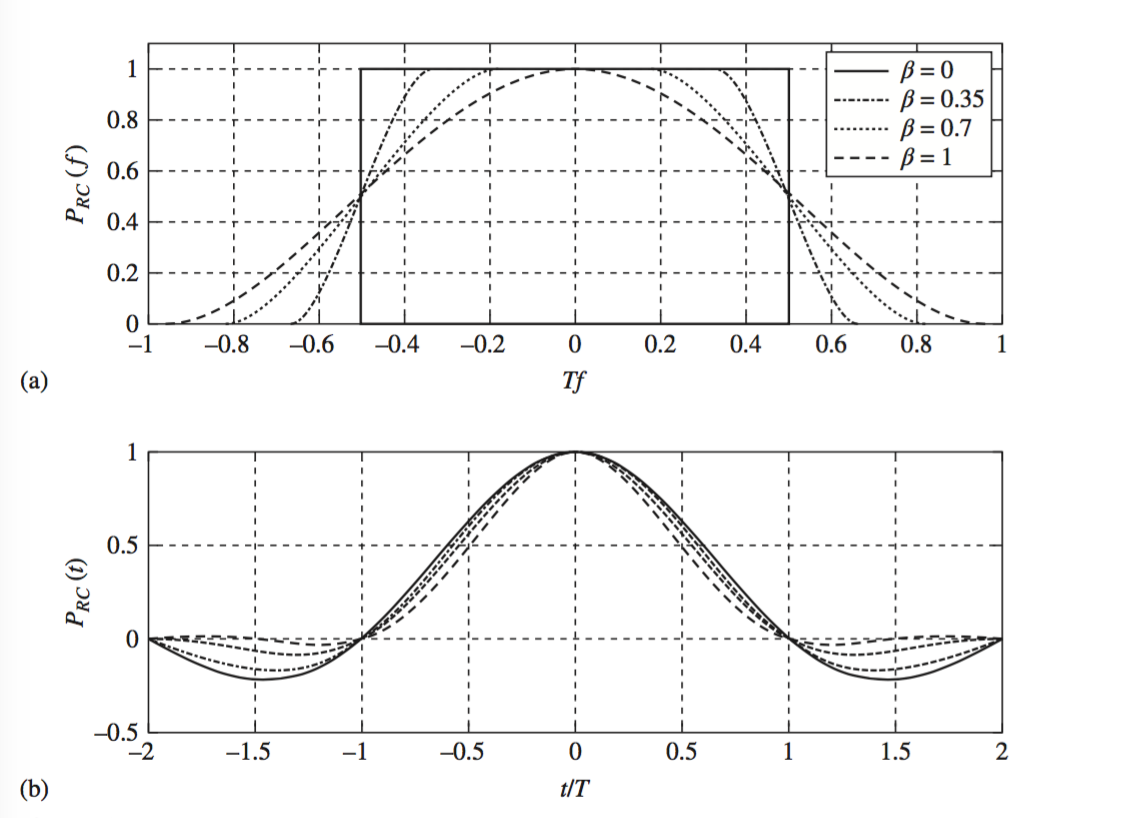
\includegraphics[width=0.8\textwidth]{isi.png}
			\end{figure}
			\end{frame}
	
			\begin{frame}
			\frametitle{Nyquist's Pulse- Shaping Criterion}
			\begin{itemize}
			\item Having a F.T of p(t), results in a pulse-shape function with sample values;
			\item a
			\[
    p(nT) = \left\{\begin{array}{lr}
        1, & \text{for } n\leq 0\\
        0, & \text{for } 0\leq n\leq inf
        \end{array}\right\} 
  \]
  			\end{itemize}
			\end{frame}
			
  			\begin{frame}
			\frametitle{Transmitter and Receiver Filters for Zero ISI}
			\begin{itemize} 
			\item Considering simplified transmitter model under consideration here, k-th sample value multiplies a unit impulse occuring at time kT and this weighted impulse train is the input to a transmitter filter with impulse response $h_t(t)$ and corresponding frequency response $H_T(f)$
			\item We can mathematically explain by following calculations,  $x_(t)$=$\sum_{k=-\infty}^{\infty} a_k*\delta(t-kT)*h_T(t) $
			\item So output of the channel will be: $y(t)= x(t)*h_c(t)$
			\item And the output of the receiver filter is : $v(t)=y(t)*h_r(t)$
			\item  We want output to have the zero-ISI property and, to be specific set: $V(t)$=$\sum_{k=-\infty}^{\infty} a_k*a_k*A_pRC(t-kT-t_d) $
			\end{itemize}
			\end{frame}
			
			\begin{frame}
			\frametitle{Figures}
			\begin{figure}
			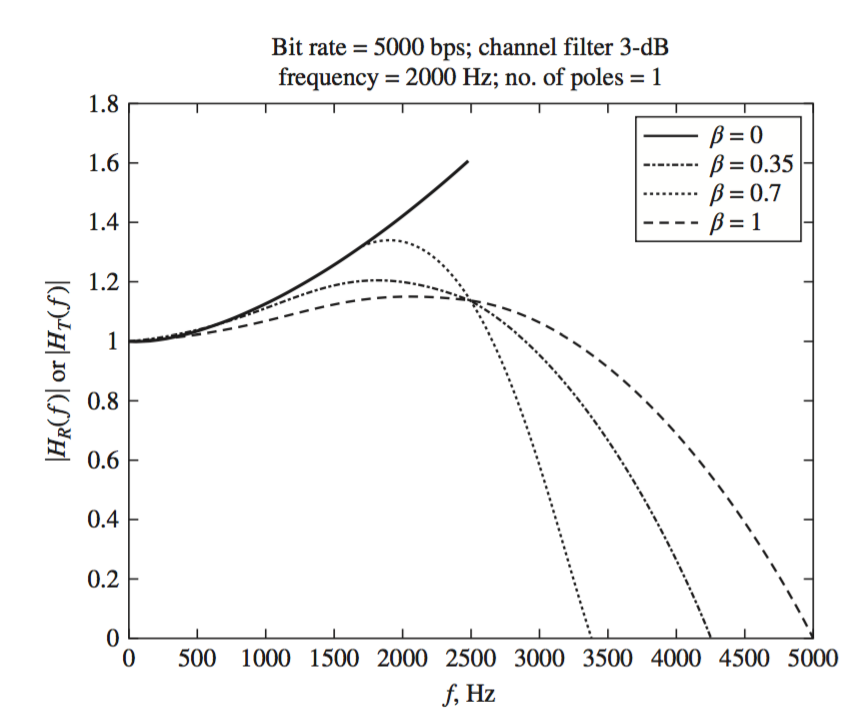
\includegraphics[width=0.8\textwidth]{54.png}
			\end{figure}
			\end{frame}
					
			\end{document}
